\section{Methods}\label{sec:methods}

\subsection{Scope and implemented architecture}
We verified a reference implementation for structured pre-consultation using
synthetic patients. The outcomes concern data interchange, interview-to-write-back
completion, model replacement, and local concurrency. Diagnostic and triage
accuracy, clinical note quality, and comparisons with clinicians were outside scope.

The implementation combines Vue patient and clinician interfaces, a FastAPI
backend, local retrieval, and a HAPI FHIR R4 sandbox (Fig.~\ref{fig:architecture})
\citep{vueJs,fastApi,hapiFHIR,fhirR4}.
A patient invitation is exchanged for a scoped session cookie; the clinician
launcher binds patient and encounter identifiers. The separate SMART integration
surface follows a different authorization flow \citep{mandelSmartOnFhir2016,smartAppLaunch}.
These verification activities exercise text-channel HTTP APIs, not browser/OAuth launch or
voice input. Isolated verification databases and an explicit loopback development
authorization bypass separate the runs from production services.

\begin{figure}[t]\centering
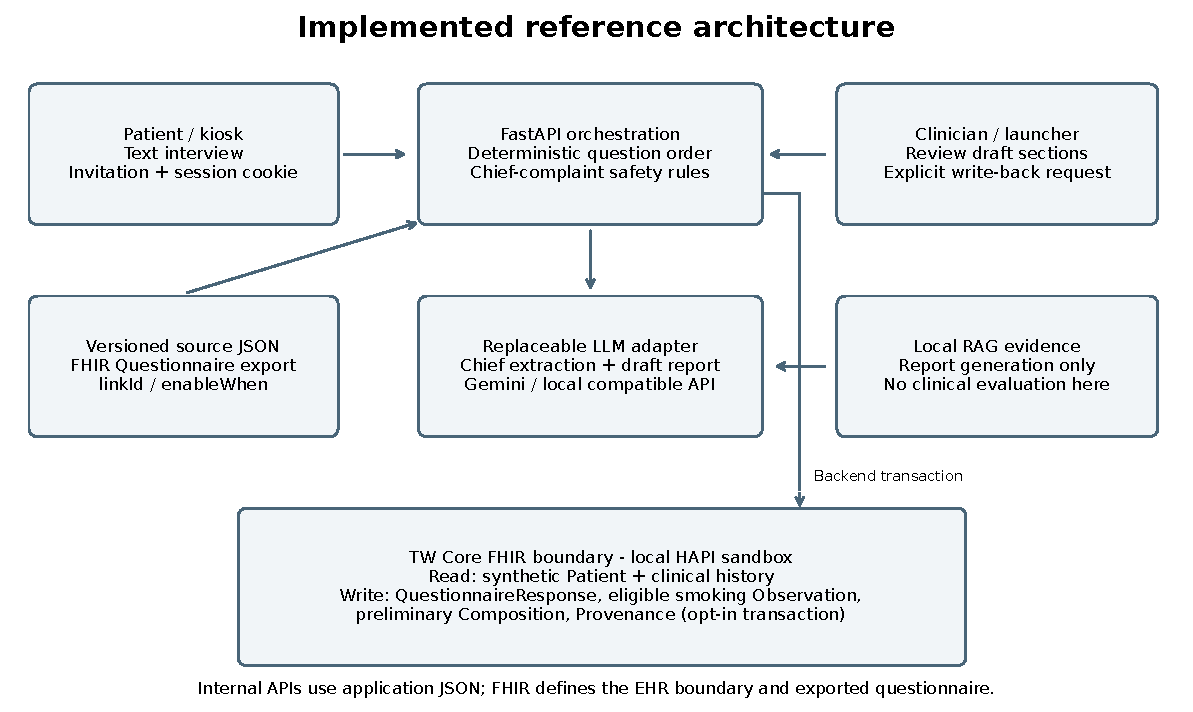
\includegraphics[width=\textwidth]{figures/fig1_architecture.pdf}
\caption{Implemented modules and data boundaries. Source JSON controls the
questionnaire engine; a corresponding FHIR Questionnaire is exported. Internal
APIs use application JSON, while FHIR defines the EHR boundary.}
\label{fig:architecture}
\end{figure}

In the default questionnaire engine evaluated here, questionnaire rules select
the next enabled question and skip EHR-prefilled fields; the LLM does not choose
the next question. An alternative engine in the code base that makes per-turn
model calls was not evaluated. Chief-complaint keywords select
the questionnaire first. Only no keyword match permits evidence-grounded model
extraction as a routing fallback. Rules and model extraction also screen the chief complaint; failed semantic assessment triggers manual handoff. At
routine completion, retrieval supplies evidence for model-generated report
sections and decision-support suggestions \citep{lewisRag2020}. These suggestions are neither
validated diagnoses nor published orders.

\subsection{Questionnaire and write-back contracts}
The encoder maps source fields to stable \texttt{linkId} values, options to coded
answers, and supported conditions to \texttt{enableWhen}. Questionnaire and
QuestionnaireResponse separate form definitions from answers \citep{fhirQuestionnaireR4,sdcIG}.
The canonical version includes a source digest and is pinned in the interview
trace when a route is selected. Write-back rejects a changed canonical version;
older records without a pin use current resolution with an explicit legacy tag.
Application extensions carry source and presentation semantics, so generic FHIR
consumers cannot assume complete runtime equivalence. The questionnaire is encoded
and published as FHIR Questionnaire, while source JSON drives execution. Tested
equivalence holds for patient-entered branching answers but diverges for
free-text EHR prefill, as quantified by R3.

Structured write-back is opt-in; Composition-only write-back remains the default.
After simulated clinician confirmation, an authorized request creates the
transaction in Table~\ref{tab:fhir}. Stable references and conditional creation
support retry idempotency. Patient, encounter, institution, and issuer checks
precede persistence. No differential-diagnosis Conditions, ClinicalImpressions,
ServiceRequests, or safety Flags are created.

\begin{table}[t]\centering\small
\caption{Write-back resources and assertion boundaries.}\label{tab:fhir}
\begin{tabular}{lp{8.1cm}}\hline
Resource & Content and boundary \\\hline
QuestionnaireResponse & Ordered answers, source markers, and the pinned canonical reference. \\
Observation & Smoking status only for an explicit mapped patient selection; EHR text is not promoted to a new patient assertion. \\
Composition & Preliminary narrative, confirmed sections, and links to structured answers. \\
Provenance & Patient informant, AI assembly, and simulated clinician-review roles; no actual clinical approval. \\\hline
\end{tabular}
\end{table}

An absent-EHR placeholder is omitted from the response. Free text outside the
option grammar is represented by the existing coded ``other'' option plus its
nested string, retaining both the original text and answer-source marker. This
avoids the validator's incompatible open-choice string/coded-condition exception
without inventing a clinical selection. The original minimal reproduction is
retained. When an answered runtime branch would lose its answer in FHIR,
write-back fails closed with a non-retryable unprocessable-content response;
unanswered branches do not create answers or block writing.

\subsection{Synthetic inputs and model disclosure}
Synthea generated the adult source cohort \citep{syntheaMethod,syntheaSoftware}.
Conversion assigns fictional Taiwanese identifiers and addresses and applies
TW Core profiles \citep{twcoreIG}. Seeds, mappings, dropped elements, and content
hashes are recorded. Taiwan-styled presentation does not establish local disease
representativeness. Input validation is separate from system-output validation.
The \ScenarioCount{} author-drafted scenarios cover chest pain, headache, and
abdominal pain, including expected safety stops and known rule gaps. The planned
benchmark was unavailable. Separate source-level Synthea modules provide
scenario-consistent backgrounds; generated patient records are not manually
rewritten to force agreement.

Mechanical audits check conditions, medications, allergies, and smoking history.
Human approval requires two independent physician decisions against current
script hashes, including patient bindings and expected paths. At generation,
\ValidatedScriptCount{} scripts have those approvals. Model and sampling
settings and pending human QA are disclosed by role in Online Resource 1,
Section S5; full prompt texts are in Sections S1 and S5. Commercial models use the Gemini Developer API; local Gemma and
Qwen use Ollama \citep{ollamaSoftware,gemmaThree,qwenTwoFive}.
Gemini API access follows the provider interface \citep{googleGeminiAPI}.
Requested temperature is distinguished from the transmitted value: the Gemini
adapter omits temperature for the configured newer Gemini models. Provider-effective
sampling and unrecorded historical thinking settings are not inferred from defaults.
Implementation, scenario drafting, orchestration, reference checking, and manuscript
revision used AI assistance; the declarations specify the remaining author review.

\subsection{Requirements and acceptance criteria}
Table~\ref{tab:requirements} maps framework requirements to checks and generated
verdicts. E1--E5 denote verification activities. Only the E1 zero-error target,
E3 zero code-change target, and E4 request-error stopping threshold were specified
before execution. The all-match/all-pass criteria for R2--R6 and the behavioral
agreement component of R7 are requirement-defined and were applied post~hoc on
2026-10-14, after inspecting the results. They are not prospective clinical
acceptance thresholds. R0 comes from the project principal investigator's requirement for
fixed questionnaire selection; its criteria were likewise applied post~hoc on
2026-10-14. Missing evidence yields an indeterminate verdict.

\begin{table}[t]\centering\footnotesize
\caption{Requirements, criterion sources, and generated verdicts. R0 uses E2 with
E3 descriptive checks; R1/R2 use E1;
R3--R6 use E2; R7 uses E3; R8 uses E4; R9 concerns E5. R7 is reported separately
for each replacement in Table~\ref{tab:e3}.}\label{tab:requirements}
\setlength{\tabcolsep}{3pt}
% Generated; edit source results or generator, never these values.
\begin{tabular}{@{}l>{\raggedright\arraybackslash}p{4.1cm}>{\raggedright\arraybackslash}p{4.3cm}p{2.3cm}@{}}
\hline
ID & Requirement & Criterion source & Verdict \\[4pt]
\hline\noalign{\vskip 3pt}
\multicolumn{4}{@{}>{\raggedright\arraybackslash}p{10.7cm}@{}}{\revadd{\textbf{E1} --- FHIR conformance and read-back: \EOneTemplatedSessions{} templated sessions, \EOneScenarioSessions{} E2 sessions, and \EOneObservationSessions{} smoking write-back sessions}} \\[3pt]
R1 & TW Core structural/profile checks & Prespecified zero errors; no validator exceptions & Pass \\[3pt]
R2 & Write/read-back identity & Requirement-defined, applied post~hoc & Pass \\[3pt]
\multicolumn{4}{@{}>{\raggedright\arraybackslash}p{10.7cm}@{}}{\revadd{\textbf{E2} --- End-to-end sessions: \ScenarioCount{} scripted scenarios $\times$ \ETwoRepeats{} repetitions with an LLM-simulated patient}} \\[3pt]
R0 & Questionnaire rules select the next question & Principal investigator requirement; criteria applied post~hoc & Pass \\[3pt]
R3 & Top-level path matches the FHIR Questionnaire & Requirement-defined, applied post~hoc & Pass \\[3pt]
R4 & Extracted-fact traceability & Requirement-defined, applied post~hoc & Pass \\[3pt]
R5 & Scripted safety-rule execution & Requirement-defined, applied post~hoc & Fail \\[3pt]
R6 & End-to-end completion without handoff & Requirement-defined, applied post~hoc & Pass \\[3pt]
\multicolumn{4}{@{}>{\raggedright\arraybackslash}p{10.7cm}@{}}{\revadd{\textbf{E3} --- Model replacement: E2 scripts rerun with the alternate commercial and local open-weight configurations}} \\[3pt]
R7 & Configuration-only substitution retaining default behaviour & Prespecified zero code lines; default-equivalence applied post~hoc & Alternate: Pass\newline Local: Fail \\[3pt]
\multicolumn{4}{@{}>{\raggedright\arraybackslash}p{10.7cm}@{}}{\revadd{\textbf{E4} --- Local load replay of E2 turns: mock model at \ELoadMockConcurrency{} and real model at \ERealConcurrency{} concurrent sessions}} \\[3pt]
R8 & National peak-load capacity & No national-demand criterion available & Not verifiable \\[3pt]
\multicolumn{4}{@{}>{\raggedright\arraybackslash}p{10.7cm}@{}}{\revadd{\textbf{E5} --- MOHW exchange-hub integration}} \\[3pt]
R9 & MOHW hub interoperability & Access prerequisite unavailable & Blocked \\[3pt]
\hline
\end{tabular}

\end{table}

\subsection{Verification activities}
R0 requires all saved system-model call tasks to concern chief extraction (at most
once per session), report generation, or RAG translation, and each script's
repeated runtime paths to be identical. Static source inspection identifies the
pure next-question selector; E3 cross-model paths are reported descriptively.
Usage records are bounded and explicitly incomplete, so this audit does not
claim a complete history of all model calls (Online Resource 1, Sections S1 and S6).

E1 uses the pinned HL7 validator with TW Core and generated questionnaire and
extension definitions \citep{hl7Validator,twcoreIG}. R1 requires zero errors and
zero validator exceptions in written resources from the templated and E2
cohorts. Structural/profile checks use \texttt{-tx n/a}; they do not establish
terminology resolution. R2 requires substantive write/read-back identity after
excluding specified server metadata and assigned identifiers. Missing outcomes
cannot count as passes. Input validation is separate, and the supplemental E1
cohort is counted only once. Online Resource 1, Sections S3 and S7, documents
these procedures.

E2 exercises invitation, text dialogue, report generation, simulated clinician
confirmation, write-back, and read-back. A distinct local Qwen model plays the
patient from scenario facts, following prior use of LLM-simulated patients in
conversational evaluation \citep{tuConversationalDiagnosticArtificial2025,johriCraftMd2025,schmidgallAgentClinic2024}. Invalid constrained answers receive an explicit
unknown fallback, never an expected-answer substitution.
R3 compares the presented top-level runtime path with the FHIR
\texttt{enableWhen} path derived primarily from the written
QuestionnaireResponse, including EHR-prefilled answers. The recorded prefilled
field list retains the skip context, including no-data fields omitted from QR.
Nested \texttt{<linkId>.other} answer details are not separate questions.
Reconstruction from runtime answer strings and the original script-derived check
are secondary evidence. Expected chief stops are excluded; unexpected stops fail.
R4 requires all persisted chief-complaint facts, including those with missing
evidence, to be traceable to patient utterances. R5 requires every scripted
red-flag rule expectation and every non-red-flag expectation to hold. This tests
rule execution, not clinical sensitivity or specificity. R6 requires write-back
and an explicit \texttt{completed} or \texttt{summary\_ready} workflow; expected
chief stops and successful retries qualify, while manual handoff does not.

E3 substitutes model configuration while retaining executable fingerprints.
R7 requires zero code changes and equality with the default configuration in
R1--R6 verdicts and per-script completion, path, and red-flag results. Shared R3 representation differences and R5
rule gaps are therefore retained in the comparison baseline. This relative
criterion does not require either configuration to pass every absolute
requirement. One-time adapter implementation is documented separately against
base commit \texttt{\AdapterBaseCommit} in Online Resource 1, Section S6.

E4 replays recorded turns with fixed-latency mock responses or real models on
backend v0.18.0 with one worker. Its prespecified stopping rule is request error
rate above \ELoadStopThreshold{}; session failure is a distinct endpoint. This
local stopping rule does not define national capacity. E5 requires access to the
MOHW exchange hub. Source hashes and frozen run selection generate all result
macros, tables, and figures; repetitions are not independent clinical observations.

\section{Results}\label{sec:results}

\subsection{R0: deterministic question selection}
R0 is \textbf{\RZeroVerdict{}}. All \ETwoDetCalls{} saved calls satisfy the task
restriction, with at most \ETwoDetChiefMax{} chief-extraction call per session;
\ETwoDetUsageIncomplete{} usage records declare incomplete coverage.
All \RZeroStableScripts{} scripts have identical paths across
\RZeroRepeats{} E2 repetitions. E3 alternate Gemini matches default paths in
\EThreeAlternateDetSamePaths{}/\EThreeAlternateDetComparedScripts{} scripts;
Gemma matches in \EThreeLocalDetSamePaths{}/\EThreeLocalDetComparedScripts{},
with chief-stage handoffs or missed stops accounting for
\EThreeLocalDetDifferentScripts{} (Online Resource 1, Section S6).
Routing sources are \ETwoDetKeywordSources{} keyword selections,
\ETwoDetExtractorSources{} recorded extraction fallbacks, and
\ETwoDetUnknownSources{} unrecorded sources after expected chief stops; missing
sources are not counted as keywords.

\subsection{R1 and R2: written resources and read-back}
R1 is \textbf{\ROneVerdict{}} and R2 is \textbf{\RTwoVerdict{}}.
Across \EOneTemplatedSessions{} templated and \EOneScenarioSessions{} E2 sessions,
\EOneResources{} written resources have \EOneErrors{} structural/profile errors
and \EOneValidatorCrashes{} validator exceptions under \texttt{-tx n/a}; all
captured submissions match their read-back counterparts
(Tables~\ref{tab:e1} and~\ref{tab:e1workflow}). All
\EOneQuestionnaireResponses{} QuestionnaireResponses have explicit outcomes,
with \EOneQRErrors{} errors and \EOneQRUnverified{} unverified responses.
The \EOneWarnings{} retained warnings comprise \EOneProvenanceWarnings{}
Provenance terminology warnings and \EOneCompositionWarnings{} Composition
narrative warnings. The unavailable pinned participant-type CodeSystem version
remains a terminology limitation, not a resolved binding.
Input-cohort checks and the templated manual-handoff case are documented
separately in Online Resource 1, Sections S3, S6, and S8.

\begin{table}[t]\centering
\caption{E1 written-resource verification. Input checks are excluded; exceptions
would prevent acceptance.}\label{tab:e1}
\footnotesize\setlength{\tabcolsep}{3pt}
% Generated; edit source results or generator, never these values.
\begin{tabular}{llllll}
\hline
Cohort & Resource & $n$ & With errors & Errors & Warnings \\
\hline
Templated cohort & Composition & 200 & 0 & 0 & 200 \\
Templated cohort & Observation & 197 & 0 & 0 & 0 \\
Templated cohort & Provenance & 200 & 0 & 0 & 800 \\
Templated cohort & QuestionnaireResponse & 200 & 0 & 0 & 0 \\
Scenario cohort & Composition & 150 & 0 & 0 & 150 \\
Scenario cohort & Observation & 100 & 0 & 0 & 0 \\
Scenario cohort & Provenance & 150 & 0 & 0 & 600 \\
Scenario cohort & QuestionnaireResponse & 150 & 0 & 0 & 0 \\
\hline
\end{tabular}

\end{table}
\begin{table}[t]\centering
\caption{E1 workflow and semantic round trip. Read uses all sessions; write uses
attempted writes; read-back uses returned references; round trip uses all captured
submissions, including those without read-back.}\label{tab:e1workflow}
\scriptsize\setlength{\tabcolsep}{3pt}
% Generated; edit source results or generator, never these values.
\begin{tabular}{llllll}
\hline
Cohort & Sessions & Read & Write & Read-back & Round-trip \\
\hline
Templated cohort & 200 & \shortstack{100.0\%\\(200/200)} & \shortstack{100.0\%\\(200/200)} & \shortstack{100.0\%\\(797/797)} & \shortstack{100.0\%\\(797/797)} \\
Scenario cohort & 150 & \shortstack{100.0\%\\(150/150)} & \shortstack{100.0\%\\(150/150)} & \shortstack{100.0\%\\(550/550)} & \shortstack{100.0\%\\(550/550)} \\
\hline
\end{tabular}

\end{table}

\subsection{R3--R6: questionnaire, evidence, rules, and completion}
R3 is \textbf{\RThreeVerdict{}}: written-FHIR paths match in
\ETwoWrittenPathAgree{}/\ETwoWrittenPathCompared{} comparable sessions, versus
\ETwoFixtureActualPathAgree{}/\ETwoFixtureActualPathCompared{} using runtime
answer strings. Failures occur in \RThreeFailingScripts{}; all first divergences
expect \texttt{chronic\_detail} but observe \texttt{past\_meds}.
Patient-entered branch controls agree in
\ETwoWrittenPathPatientControllerAgree{}/\ETwoWrittenPathPatientControllerCompared{},
whereas EHR-prefilled controls agree in
\ETwoWrittenPathEhrControllerAgree{}/\ETwoWrittenPathEhrControllerCompared{}
(Online Resource 1, Section S6.3). R4 is \textbf{\RFourVerdict{}}, with fact traceability of
\ETwoTraceability{}. R5 is \textbf{\RFiveVerdict{}}: the failing scripts are
\RFiveFailingScripts{}, exposing existing rule gaps rather than a transport
failure. The full red-flag and non-red-flag denominators appear in Online
Resource 1, Section S6.
R6 is \textbf{\RSixVerdict{}}, with completion of \ETwoCompletion{}, including
\ETwoChiefStopsCompleted{} expected chief stops and
\ETwoTimeoutCompleted{} recovery after a timeout and retry.
The simulated-patient fixture has answer biases, but verbatim chief complaints,
separate runtime/FHIR path checks, and content-independent structure/read-back
checks distinguish fixture bias from the representation discrepancy (Online Resource 1, Section S6.3).

\subsection{R7: configuration-only replacement}
R7 is \textbf{\EThreeAlternateSwapVerdict{}} for alternate Gemini and
\textbf{\EThreeLocalSwapVerdict{}} for local Gemma
(Table~\ref{tab:e3}). The configurations retained identical executable
fingerprints with no code changes during replacement. Alternate Gemini retains
the default requirement verdicts and per-script outcomes, including the shared
R3 and R5 failures; this is behavioral agreement with the default, not absolute safety
acceptance. The local replacement differs on
\EThreeLocalSwapFailingScripts{}: \EThreeLocalRSixFailingScripts{} enter manual
handoff after chief-assessment timeouts, while \EThreeLocalAdditionalSafetyFailingScripts{}
miss expected red-flag stops.
Late worker completion does not reverse a handoff. Full per-session evidence is
in Online Resource 1, Sections S6 and S7.

\begin{table}[t]\centering\footnotesize
\caption{E3 requirement verdicts by configuration. R7 compares each replacement
with the default, including per-script completion, path, and red-flag outcomes;
shared rule gaps do not themselves fail this relative check. Code lines exclude
one-time adapter implementation.}\label{tab:e3}
\setlength{\tabcolsep}{3pt}
% Generated; edit source results or generator, never these values.
\begin{tabular}{@{}lp{3.2cm}p{3.2cm}p{3.2cm}@{}}
\hline
Check & Default Gemini & Alternate Gemini & Local Gemma 3 \\[4pt]
\hline\noalign{\vskip 3pt}
R1 & Pass & Pass & Pass \\[3pt]
R2 & Pass & Pass & Pass \\[3pt]
R3 & Pass & Pass & Fail \\[3pt]
R4 & Pass & Pass & Pass \\[3pt]
R5 & Fail & Fail & Fail \\[3pt]
R6 & Pass & Pass & Fail \\[3pt]
Code lines & 0 & 0 & 0 \\[3pt]
R7 & Reference & Pass & Fail \\[3pt]
\hline
\end{tabular}

\end{table}

\subsection{R8 and R9: unavailable acceptance evidence}
R8 is \textbf{\REightVerdict{}} because national peak demand remains
\texttt{TODO\_PEAK\_DEMAND}. The local request-error stop condition cannot
substitute for a national-demand criterion. R9 is \textbf{\RNineVerdict{}}
because exchange-hub access is unavailable; E5 has no measured result.
Timing, turns, tokens, bounded cost estimates, fact counts, and local load
observations are descriptive background in Online Resource 1, Section S6.

\section{Discussion}\label{sec:discussion}
R0 and R3 distinguish stable selection from agreement between representations.
Runtime JSON uses fixed substring conditions on free-text EHR values; FHIR
write-back encodes unrecognized text as coded ``other'' with nested original
text, enabling \texttt{chronic\_detail} in the published Questionnaire.
These fixed rules disagree without any AI decision, even though repeated
runtime paths are identical. Clinicians must decide whether out-of-option EHR
text should trigger follow-up before the rules are unified; this work changes
neither rule set. Passing structural and read-back checks does not establish
branch equivalence or clinical meaning.

R5 failure identifies unmet rule expectations in \RFiveFailingScripts{},
including suspected pulmonary embolism and abdominal aortic aneurysm without syncope.
Only chief-complaint screening runs in the default engine; later questionnaire
answers do not trigger renewed screening. Other known code-level limitations
include sustained exertional pressure without diaphoresis or syncope,
prefill-dependent structured ectopic-pregnancy matching, and overly broad raw
negation windows. These require qualified clinical review; no rules were changed.

R7 distinguishes configuration compatibility from preserved behavior. Agreement
with a default that fails R3 and R5 cannot establish representation equivalence
or clinical safety. Gemma's handoffs
and missed scripted stops fail the relative replacement criterion. Traceability
over surviving extracted facts also cannot establish extraction coverage; the
retention and timeout diagnostics remain in Online Resource 1, Section S6.
R8 requires externally supplied demand and a justified acceptance criterion;
local load observations do not establish national readiness. R9 requires an
authorized exchange-hub environment before verification can proceed.

\subsection{Limitations and clinical review needs}
All scenario-based verdicts are provisional pending physician review and
independent transcript/fact audits. Requirements were organized after viewing
the results, and requirement-defined criteria are explicitly labeled post hoc.
Synthetic demographics are not representative, evidence spans do not validate
clinical interpretation, and clinician confirmation was simulated.
EHR prefill can retain social/contextual Condition text and English labels in
Chinese forms; faithful encoding does not make that mapping clinically
appropriate (Online Resource 1, Section S3).
The sandbox does not establish production authorization, tenant isolation,
browser SMART integration, diagnostic accuracy, clinical utility, or deployment
readiness. Terminology review, institutional governance, and human approval
remain separate prerequisites.

\section{Conclusion}\label{sec:conclusion}
The absolute requirements \PassingRequirements{} pass; \FailingRequirements{}
fail within the defined software-verification scope. Deterministic question
selection does not guarantee agreement between runtime and written FHIR branching.
R7 is \EThreeAlternateSwapVerdict{} for alternate Gemini, retaining default
outcomes including shared R3/R5 failures, and \EThreeLocalSwapVerdict{} for Gemma.
National peak capacity is \REightVerdict{} and exchange integration is
\RNineVerdict{}. Checks retain \texttt{-tx n/a}, without terminology resolution;
simulated clinician confirmation and provisional scenarios do not establish
clinical validation or deployment readiness.

\backmatter
\bmhead{Supplementary information}
Online Resource 1 (\texttt{ESM\_1.pdf}) provides system and prompt details
(Section S1), FHIR examples (S2), synthetic conversion (S3), provisional scenarios
(S4), model disclosure (S5), complete results and a provisional walkthrough
(S6), harness procedures (S7), validator limitations (S8), and version locks (S9).
Online Resource 2 (\texttt{ESM\_2.zip}) contains the corresponding machine-readable
scripts, review materials, FHIR examples, synthetic sample bundles, prompts,
configurations, summaries, and a hash manifest. No scenario is physician-approved;
the walkthrough remains provisional and the clinician screenshot is pending.

\bmhead{Acknowledgements}
Author confirmation of acknowledgements and institutional wording is pending.

\section*{Declarations}
\textbf{Funding, competing interests, and contributions.} Authors must supply and
verify these statements and final approval.\par
\textbf{Ethics and consent.} Only synthetic data were used. Authors must confirm
the applicable institutional determination; no ethics approval is asserted.\par
\textbf{Data availability.} Online Resource 2 contains provisional synthetic
scripts, review materials, sample TW Core bundles, FHIR examples, selected result
summaries and manifests, and configuration/prompt provenance. Full session records
and RAG source text are excluded. Medscape \citep{medscapeReference} redistribution rights require author
confirmation (\texttt{TODO\_AUTHOR}).\par
\textbf{Code availability.} Reproduction commands and source paths accompany
Online Resource 2; the public repository location, archival identifier, and code/data
licenses remain \texttt{TODO\_AUTHOR}.\par
\textbf{AI assistance.} Claude Code and Codex assisted code and scenario drafting,
verification orchestration, source checking, and manuscript drafting and revision.
The authoring log records Claude Code with \texttt{claude-opus-5-5} and
Codex in the GPT-6 family; exact tool releases and Codex runtime version remain
unrecorded. Authors must confirm these details and the final disclosure
wording (\texttt{TODO\_AUTHOR}; Online Resource 1, Section S5). Authors must verify citations, review technical and clinical content,
and approve the final text; scenario approvals and independent audits remain pending.

\bibliography{sn-bibliography}
